
\chapter{Evaluation} 
% How good is your solution? How well did you solve the general problem, and what evidence do you have to support that?

In this chapter, we shall outline the evaluation process and discuss results. First, we shall examine how evaluation was undertaken, including details on our experiments and user survey. Then, we shall show the results from both these evaluations. Finally, we shall discuss these results and present an argument based on the evidence garnered.

\section{Experiments Design}

Our experiments to gather quantitative (and some qualitative) data shall be undertaken on a simulated network; this shall be built using Mininet on a Ubuntu virtual machine. These experiments shall be conducted on all of our builds. 

For our WebTransport experiments, our network topology consists of two hosts, two switches and a server - this is illustrated by Figure \ref{perfect-topology-wt}.

\begin{figure}[h]
    \centering
    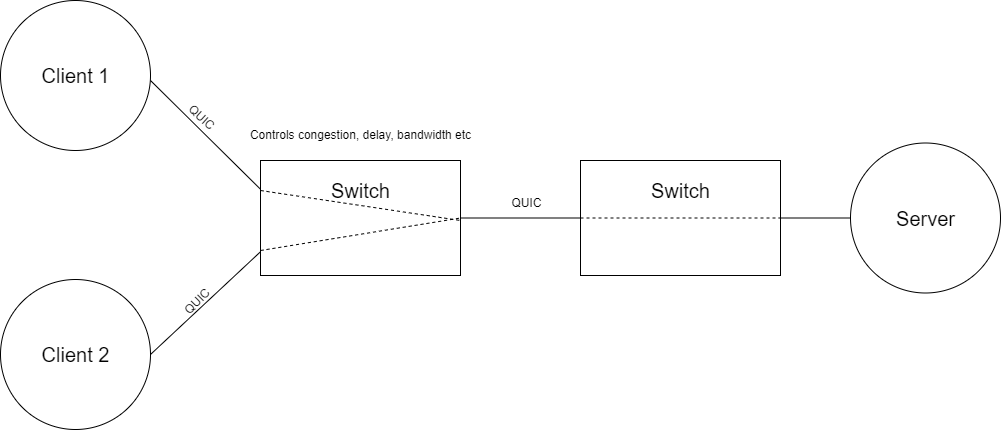
\includegraphics[width=0.8\columnwidth]{images/perfect-topology.png}
	\caption{A "perfect" network topology used to test our WebTransport builds.}
    \label{perfect-topology-wt}
\end{figure}

We can consider this network topology to be "perfect" as it has no competing traffic and therefore theoretically no congestion in the switches between nodes. This is not ideal for replicating realistic network conditions - however, as our WebTransport builds are likely to have varying performance in even perfect conditions, we can still effectively evaluate the builds in this perfect environment. We would suggest that further work could be done here to evaluate the WebTransport builds in a non-perfect simulated network, but due to time constraints we shall not do so in this project.

For our WebRTC experiments, our network topology shall consist of two hosts directly, one switch and two servers. We have one server that hosts PeerJS, and one that hosts socket.io. This topology is illustrated by Figure \ref{perfect-topology-webrtc}.

\begin{figure}[h]
    \centering
    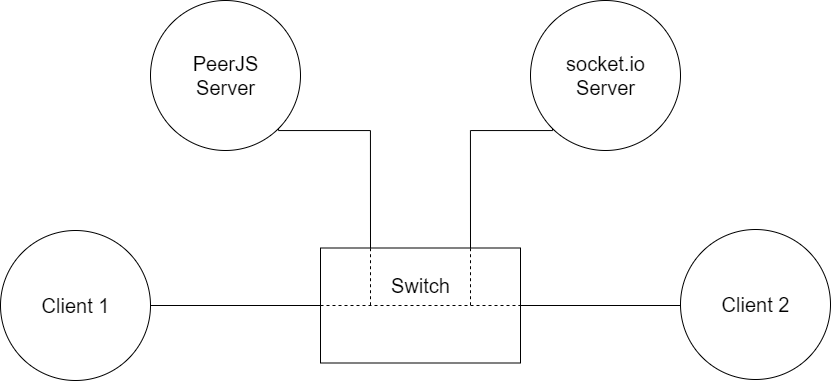
\includegraphics[width=0.7\columnwidth]{images/p2p-topology.png}
	\caption{A "perfect" network topology used to test our WebRTC builds.}
    \label{perfect-topology-webrtc}
\end{figure}

This topology has the same issue as our WebTransport topology in that it's "perfect". However, as we need to compare our WebRTC build to our WebTransport build, we must do so in the same network conditions to ensure the soundness of our experiments, so we shall continue to use these perfect conditions. Additionally, we shall disable audio data in our WebRTC build for the same reason.

Once these topologies have been built, we can experiment on our builds. The method is similar for both the WebTransport and WebRTC builds, with some slight variation to account for the different technologies. 

For our WebTransport builds, we first introduce lists of independent variables we wish to alter. Then, the network topology is adjusted based on the first items in these lists of independent variables. Following this, we automate the transmission of data between our two clients by using Selenium and the Mininet Python API to launch two instances of Google Chrome. During these transmissions, we use alternate builds that natively log relevant data and terminate once an arbitrary amount of packets (we send 1000 packets) has been sent. After these packets have been sent by the second client, the connection closes and relevant data is printed from our clients to Chrome's console log - this output is then fed into a CSV file and parsed. Then, the Mininet topology is shut down and the process repeats for the next set of independent variable values. Once the independent variable lists have been exhausted,  the outputted CSV data is analysed and, if necessary, parsed by matplotlib to generate visualisations that allow us to draw conclusions. 

The experiments for our WebRTC builds work very similarly, with some slight differences relating to the collection of relevant data and the Selenium automation of our clients. Instead of manually calculating the desired dependent variables from within our clients, we utilise the WebRTC Statistics API \cite{webrtc-stats-api}. From this API, we utilise the \textit{RTCInboundRtpStreamStats} dictionary \cite{webrtc-stats-api-inboundrtpstats}, and specifically the following measurement metrics: \textit{totalDecodeTime}, \textit{framesDecoded}, \textit{framesReceived},
\textit{packetsReceived}, \textit{packetsLost}, \textit{framesReceived} and \textit{framesDropped}. These metrics are collected on one of the two clients and outputted as before. Because the WebRTC builds are more stable, we chose to send 10000 packets rather than 1000 in order to have a greater chance of catching the occurrence of anomalies. Important dependent variables such as decoding time and loss are not affected by this decision, as decoding time is an average value and loss is a percentage.

As our primary aim is to evaluate WebTransport, WebRTC and the underlying data transfer methods rather than QUIC, SRTP and HTTP/3, measurements take place exclusively at our client endpoints. There is no notion in our results of how the data is transferred via the transport protocols. We had attempted to include some evaluations of QUIC for argument's sake, but ran into several difficulties. Our main issue was due to the way QUIC encrypts as much data as possible - it was not possible to extract meaningful data from packets sent between nodes as it was all encrypted. One solution to this may have been utilising qvis and qlog; these are tools specifically developed to work around this issue. However, qvis and qlog are in early stages of development and documentation is sparse - after attempting to get it to work, we decided to drop this aspect of experimentation and focus solely on WebTransport and WebRTC. In future work, it may be interesting to evaluate QUIC as well as WebTransport (and by extension, SRTP as well as WebRTC) and see if the API hinders or aids the transport protocol's performance in any way.

We shall now outline each of the performed experiments, highlighting independent and dependent variables, aims and expected results of each. The following experiments shall be conducted on all of our builds.

\subsection{The Experiments}

In total, we conducted five experiments on our WebTransport and WebRTC builds. In the following experiment descriptions, there are several definitions we must define. "Perceived latency" shall refer to how long it takes a frame to be fully processed by a client after the first packet of that frame is sent from the other client. "Actual latency" refers to how long it takes for a packet to be received by a client after being sent from the other client. "Decoding time" refers to the time difference between perceived latency and actual latency - this shall demonstrate how long it takes the receiving client to process a frame after the first packet of that frame is received. It should be noted that actual and perceived latency shall not be measured in our WebRTC builds. This is because it is not possible via the WebRTC Statistics API and we cannot develop an alternative solution within the timescale of our project - we can instead measure decoding time by dividing the amount of frames decoded by the total amount of frames received (both of these metrics are measured by the WebRTC Statistics API).

The dependent variables measured in each experiment are the same: perceived latency, actual latency, decoding time, packet loss (not measured in our WebTransport Streams build) and image quality. We chose these variables as we identified that these metrics are the most affected by adverse network conditions and also the most important to the end user experience. If any of these metrics are too high, the builds are likely suffering significantly and the user experience is probably degraded.  Although image quality is qualitative and therefore less precise, it is still a useful metric as it gives a simple indication of how the user experience is being affected.

The experiments are as follows.
\hfill{}\\
\subsubsection*{Bandwidth}
\hfill{}\\
Here, the independent variable is the bandwidth of the topology links. This experiment is important as it allows us to observe specifically how our builds cope with varying bandwidth. 
The expectation from this experiment is that, for all builds, both latencies worsen as bandwidth decreases, but packet loss will stay either the same or improve. We expect this effect to be particularly significant on the WebTransport Datagrams build where decreased bandwidth would result in there being more time for the client queue to accept late datagrams.
\hfill{}\\
\subsubsection*{Loss}
\hfill{}\\
Here, the independent variable is the loss percentage of the topology links. We expect that as it gets to extreme packet loss, both WebTransport builds will suffer extensively. In particular, the Datagrams build will output extremely poor image quality as we do not expect the code that deals with packet loss to operate well. We do not expect the Streams build to suffer in terms of image quality as streams are lossless, but latency may increase significantly as data is retransmitted more than usual. We expect that WebRTC will suffer slightly, but maintain decent image quality thanks to its forward error correction mechanisms.
\hfill{}\\
\subsubsection*{Latency}
\hfill{}\\
Here, the independent variable is the latency of the topology links. The aim of this experiment is to find out where WebTransport's bottleneck is - it will be interesting to see at what point the latency is too large for the packet reordering code to fall apart and discard too many packets. We do not expect the WebTransport Datagrams builds to cope well as latency increases. We expect that the Streams build and the WebRTC build will cope with respect to image quality, but the delay will be significant enough to degrade user experience.
\hfill{}\\
\subsubsection*{Network Quality (Bandwidth, Loss and Latency)}
\hfill{}\\
Here, the independent variables are the bandwidth, loss and latency of the topology links. The aim of this experiment is to simulate how WebTransport and WebRTC will perform on different qualities of network. We expect that the WebTransport builds will perform extremely poorly in bad network conditions, whereas the WebRTC build will likely maintain decent quality. In particular, the WebTransport Datagrams build will suffer for the same reasons as outlined in the previous experiments, and the image quality will degrade significantly. Additionally, the Streams build's rendered images will have too high of a delay to provide a satisfactory user experience.
\hfill{}\\
\subsubsection*{CPU Usage}
\hfill{}\\
During early and informal experimentation, it was noticed that the builds, even on a simulated network with perfect metrics, did not perform as well on our virtual machine as on our computer's native OS. We suspected that our virtual machine's comparatively worse system resource allocations were throttling the performance of the builds. To investigate this, we use the CPU usage (as a percentage value) of each client host as our independent variable.

\hfill{}\\
All of these experiments will give us an overview of how WebTransport and WebRTC send, receive and process video data in different network conditions. Hopefully, they shall allow us to achieve our main goal for this project of quantitatively evaluating the performance of several builds of video conferencing application using different APIs and data transfer methods. 

\section{User Survey Design}

In order to achieve our secondary aim of answering whether or not using WebTransport makes any noticeable differences to the user experience or not, we shall undertake a user survey. The ethics approval form for this survey can be seen in Figures \ref{ethics-1} and \ref{ethics-2}. This survey shall show anonymous participants recordings of six different builds of our video conferencing application implementations. The participants shall not know what technologies or data transfer methods are utilised in each build. The first three builds are our WebTransport Datagrams, WebTransport Streams and WebRTC builds - these are all run on our native machine in a "perfect" network (i.e. no adjusted metrics). The latter three builds are the same, but shall be running on our virtual machine with latency, bandwidth and loss adjusted. In these latter cases, the topology links shall have bandwidth set to 90 Mbps (Megabits per second), loss set to 0.5\% and latency set to 12.5 ms (milliseconds); these figures were arbitrarily chosen, but were shown to output a realistic simulation in our experiments.

Participants shall be asked three questions for each recording presented to them. For each question, the user is prompted to answer on a five-point Likert scale. These questions are as follows:

\textbf{\textit{"How would you rate the image quality of the video you are receiving? Does the received video resemble the video being sent out?"}}

\textbf{\textit{"How would you rate the "smoothness" of the video you are receiving? i.e. does it stutter or lag?"}}

\textbf{\textit{"Overall, how would you rate the video you are receiving out of 5?"}}

After answering these questions for each build, the user shall be presented a recording of all six builds on one screen. They shall then be asked to rank all the builds from best to worst, with no builds both being tied for one place.

Finally, the participant shall be give an opportunity to provide any feedback or observations they make.

Receiving these answers shall give us a good indication of whether or not users can tell the difference between our different builds and utilised technologies. Furthermore, it may provide some supplementary evidence (in addition to our experiments) of how each build performs.

\section{Evidence}
In the following section, we shall go through each experiment and discuss the results before discussing the results from our user surveys.

\subsection{Experiments}

\subsubsection{Experiment 1 - Adjusting Bandwidth} 
\hfill{} \\
Table \ref{tab:wt-dg-bw} displays all the collected data during this experiment for the WebTransport Datagrams build. From this data, we can generate several visualisations to aid us in understanding how the WebTransport Datagrams build handles received datagrams.
An interesting observation to make here is that the latencies and decoding time are relatively stable until link bandwidth gets below a certain threshold - here, it increases significantly. These effects can be seen in Figure \ref{fig:dg-bw-lat} and Figure \ref{fig:all-bw-decoding}. 

\begin{figure}[h]
    \centering
    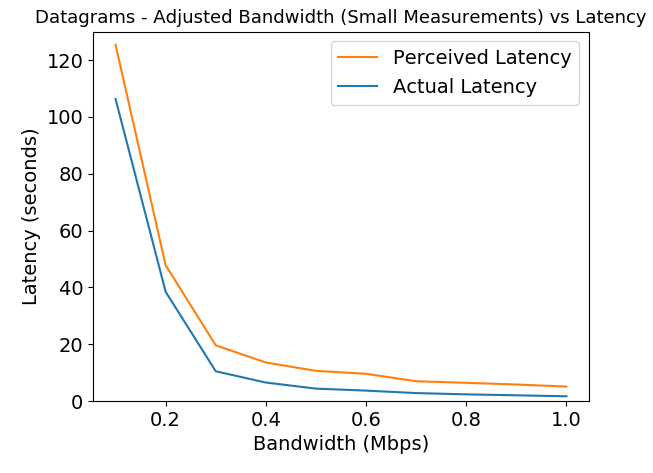
\includegraphics[width=0.52\linewidth]{images/bandwidth/dg-bw-lat-small.png}    
    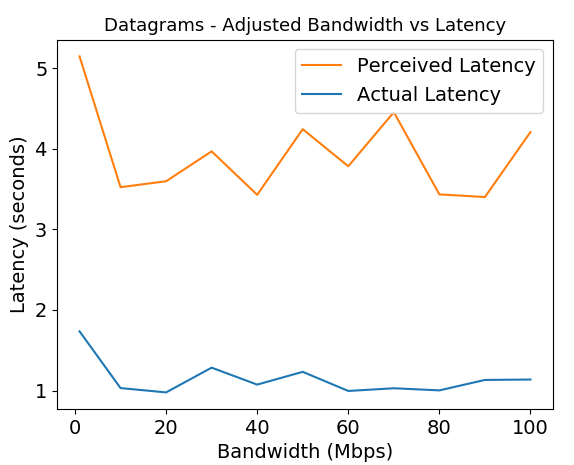
\includegraphics[width=0.46\linewidth]{images/bandwidth/dg-bw-lat.png}    
    \caption{Latencies affected by link bandwidth in the WebTransport Datagrams build.}

    % use the notation fig:name to cross reference a figure
    \label{fig:dg-bw-lat} 
\end{figure}

Throughout all our Datagrams build measurements, we can see that the perceived latency is consistently around 2-4 seconds more than the actual latency (indicating that it takes around this time to decode each frame of video data). Perceived latency (and as a result, our decoding time) is so high because our algorithms that handle packet loss and disorder are very inefficient - packets that arrive too early and are queued for significant periods of time greatly increase perceived latency and therefore decoding time. As latencies increase, the rendered output increasingly lags and image quality becomes very erratic. This same effect can be seen in our Streams build, although to less of an extent.

Table \ref{tab:wt-streams-bw} displays the results from our Streams build - loss is not measured here as streams are lossless. Figure \ref{fig:dg-streams-bw-lat} maps the Streams build's actual and perceived latencies onto the same plot as the Datagram build's. We can see that our Streams build largely follows the same trends as our Datagrams build, albeit with two significant differences. We can notice that the actual latency and perceived latency are much closer together, indicating that the decoding time of our Streams build is always far less than our Datagrams build. This makes sense as our Streams build does not have to deal with disordered or lost packets, meaning that frames can be decoded far quicker as WebTransport is able to process each packet as soon as it is received by the API. The second difference is the suddenly large latency values at the 1 Mbps mark. However, this is expected behaviour. This occurs because this threshold is the point at which the link bandwidth is smaller than the bandwidth at which our video is encoded at. To elaborate, our clients send video data of frame size 100 pixels x 100 pixels. Each pixel is equal to 1 byte, and so the total bytes it takes to transmit one frame is 10000 bytes (100 x 100). As our packets are 1024 bytes long and contain 1004 bytes of image data, it takes 10 packets to send one frame of video data (10000 ÷ 1004 = 9.96 i.e. 10 packets required). Our clients send roughly 10 frames per second, with packets constantly being sent, or "in flight". 10 frames per second means that roughly 100 packets are being sent every second, which means that approximately 102400 bytes (100 packets x packet size) are being transmitted at any one time. As we drop below the bandwidth threshold, our latencies (and consequently our decoding time) suffer as the bandwidth is often no longer able to account for the amount of packets constantly in flight.
The different thresholds for each build can be observed in Figure \ref{fig:dg-streams-bw-lat}. For our Streams build, the threshold is clearly 1 Mbps - 1 Mbps is equal to 125000 bytes, and it is feasible that packet retransmission results in this build's amount of data in flight crossing this threshold and suffering as a result. For our Datagrams build, the decline in latencies and decoding time is more gradual, but the threshold appears to be between 0.8 and 1 Mbps.

\begin{figure}[h]
    \centering
    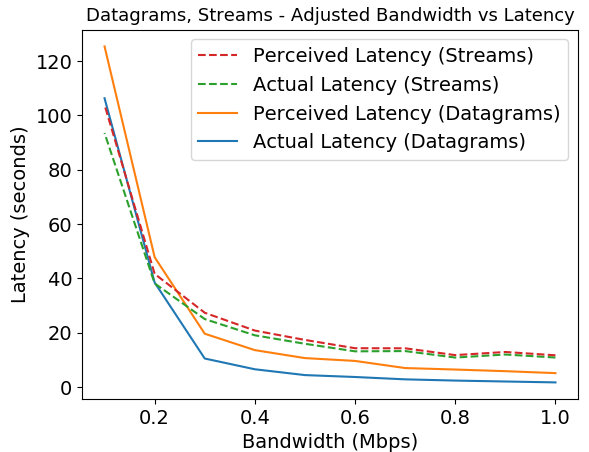
\includegraphics[width=0.49\linewidth]{images/bandwidth/dg-streams-bw-lat-small.png}  
    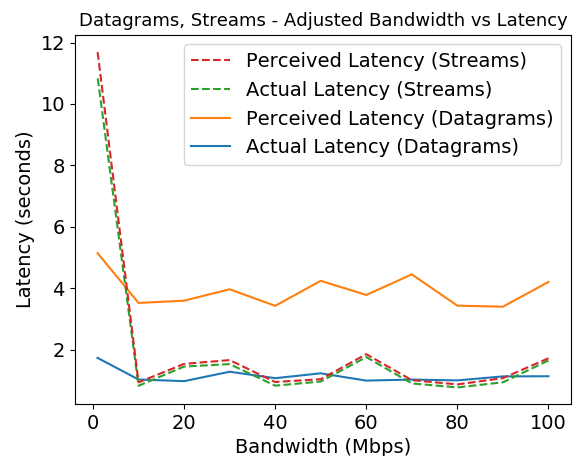
\includegraphics[width=0.49\linewidth]{images/bandwidth/dg-streams-bw-lat.png}    
    \caption{Latencies affected by link bandwidth in the WebTransport Datagrams and Streams builds.}

    % use the notation fig:name to cross reference a figure
    \label{fig:dg-streams-bw-lat} 
\end{figure}

Finally with our WebTransport builds, we can see that adjusting bandwidth does not affect application packet loss that much until we get to the same aforementioned threshold of 1 Mbps. This is displayed in Figure \ref{fig:dg-bw-loss}. This is once again, expected behaviour. The loss here is relatively insignificant, until we get to extremely low bandwidth values (between 0.1 and 0.2 Mbps).

\begin{figure}[h]
    \centering
     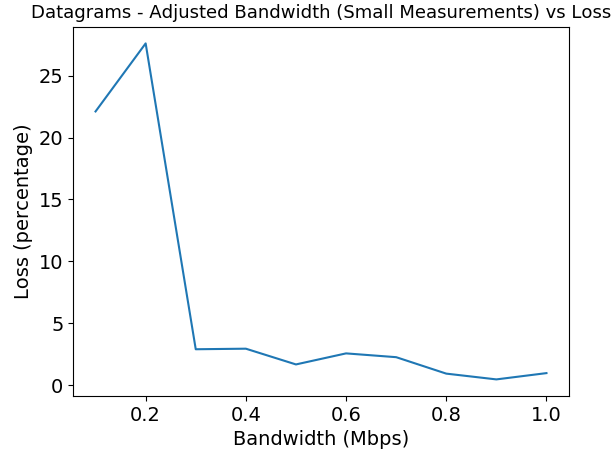
\includegraphics[width=0.49\linewidth]{images/bandwidth/dg-bw-loss-small.png}    
    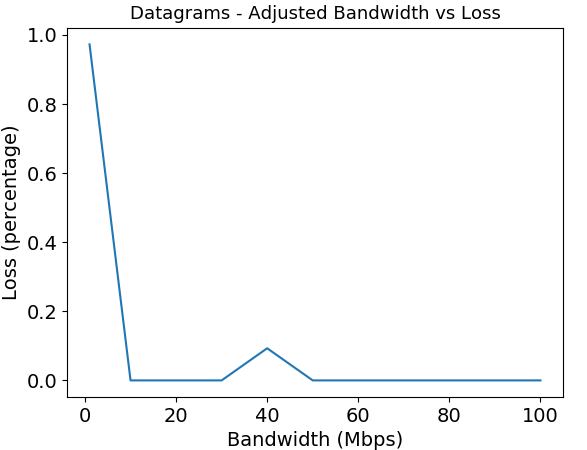
\includegraphics[width=0.49\linewidth]{images/bandwidth/dg-bw-loss.png}    
    \caption{Packet loss affected by link bandwidth in the WebTransport Datagrams and Streams builds.}

    % use the notation fig:name to cross reference a figure
    \label{fig:dg-bw-loss} 
\end{figure}

Our WebRTC builds generally fared better with respect to both decoding time and packet loss. All data gathered for this experiment can be seen in Table \ref{tab:webrtc-bw}.

We can clearly see that link bandwidth has no apparent effect on the WebRTC build. Decoding time varies slightly in apparently random fashion and frames are occasionally dropped, but there is again no discernible trend for this. Furthermore, the decoding time is far lower than our WebTransport Datagrams build, and lower than our WebTransport Streams build (particularly with extremely low bandwidth values) - this is displayed in Figure \ref{fig:all-bw-decoding}.

\begin{figure}[h]
    \centering
    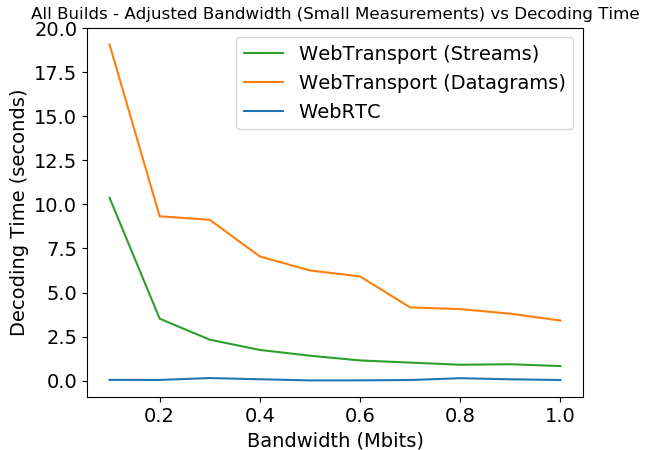
\includegraphics[width=0.51\linewidth]{images/bandwidth/all-bw-decoding-small.png}    
    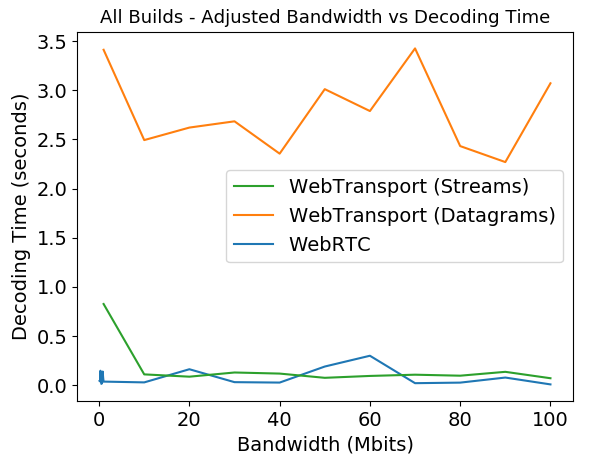
\includegraphics[width=0.48\linewidth]{images/bandwidth/all-bw-decoding.png}    
    \caption{Decoding time affected by link bandwidth in all our builds.}

    % use the notation fig:name to cross reference a figure
    \label{fig:all-bw-decoding} 
\end{figure}

Overall, it is clear to see that adjusting link bandwidth has a significant effect on our WebTransport builds' actual and perceived latencies, particularly as bandwidth values get to extreme lows. Our Streams build appears to perform slightly better than our Datagrams build in this regard, but suffers slightly sooner due to the higher amount of packets constantly in flight. Link bandwidth does not appear to affect loss in our Datagrams build that much until it gets to extreme lows between 0.1 and 0.2 Mbps. The WebRTC build handles low bandwidth extremely well, suffering very little packet loss and frame discards, and maintaining a steadily low decoding time. The WebRTC's build consistently low decoding time is likely what results in its consistently smooth video output - rendered video lags heavily when decoding time increases in our WebTransport builds.
\hfill{} \\

\subsubsection{Experiment 2 - Adjusting Latency} 
\hfill{} \\
The results from our WebTransport Datagrams build (as seen in Table \ref{tab:wt-dg-lat}) show some fairly predictable trends when increasing link latency. 
Firstly, both latencies steadily increase alongside link latency and appear to plateau between 12-16 seconds after the 100ms link latency point. There is a roughly two second decoding time throughout our measurements. This is unsurprising as, unlike the previous bandwidth experiments, the rate at which data is being received is not changed - this results in our build constantly receiving data, and therefore processing it at a constant rate. It should be noted that this experiment failed for our WebTransport Datagrams and Streams builds after 250ms, where the connection between the client and the server could no longer be established due to the server timing out. 
% \todo{insert how this is a QUIC policy}

Finally, we can see that the build performs very well in relation to packet loss until the 150ms link latency mark - here, after not losing any packets at all, we suddenly lose over half. This loss continues to increase as link latency increases; we can observe this on the left of Figure \ref{fig:dg-lat-loss-dg-streams-lat-lat}. As this sudden loss occurs, image quality sharply declines and rendered output becomes unrecognisable. It is unclear why this occurs at this specific point, but it demonstrates that the build does not handle high latency and resulting packet loss well. 

The application latencies of our WebTransport Streams build are similarly affected. The results of this experiment can be seen in Table \ref{tab:wt-streams-lat}. Decoding time is smaller than our Datagrams build until latency gets above 150ms - interestingly, the decoding time here becomes greater than our Datagrams counterpart. After this point, image quality and smoothness degrades. This high decoding time occurs due to the lossless nature of streams. As we know, if packets are lost in a streams connection, these packets are retransmitted. In this scenario, the decoding of our video frame would halt to wait for these retransmitted packets to arrive because streams deliver packets in order. In a low-latency network, this would negligibly increase decoding time - however, in high-latency networks, it takes longer for these packets to be retransmitted and decoding time consequently rises significantly. This is the main reason why streams are generally considered to be unsuitable for use in video conferencing applications. This conclusion is corroborated by Perkins' and Ott's 2018 paper that states a significant problem with QUIC's streams implementation is "media data being retransmitted once it has passed its play-out
deadline and is no longer needed" \cite{perkins2018}. 
The differences in actual and perceived latencies between the two builds can be seen on the right of Figure \ref{fig:dg-lat-loss-dg-streams-lat-lat}. From this, we can see that the Streams build is able to render video frames faster than the Datagrams build at low link latencies. However, as link latency increases and the Streams build's decoding time increases, the Datagrams build actually renders video frames faster. However, this is by a relatively slim margin (~2-4 seconds), and the image quality of both is very poor. 

% \begin{figure}[h]
%     \centering
%     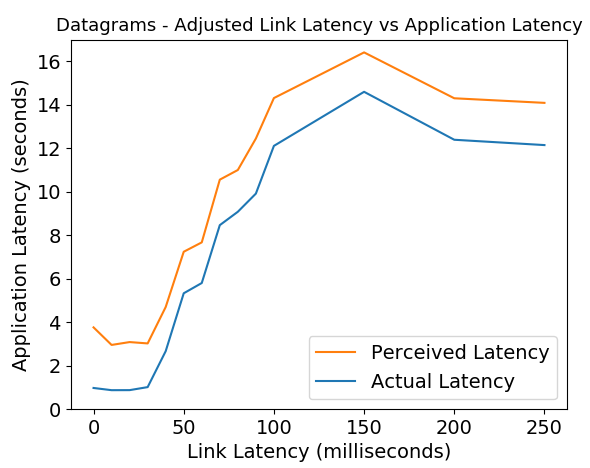
\includegraphics[width=0.49\linewidth]{images/latency/dg-lat-lat.png}
%     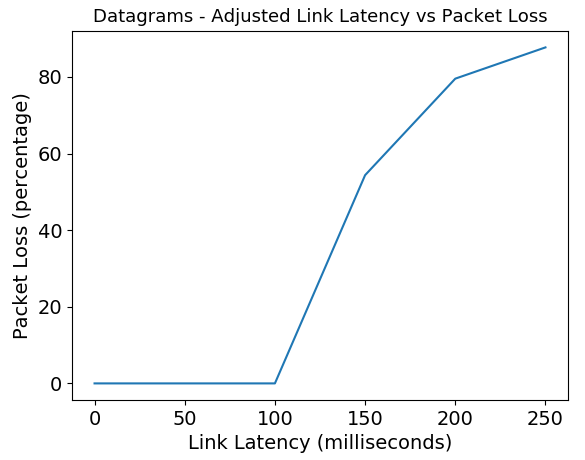
\includegraphics[width=0.49\linewidth]{images/latency/dg-lat-loss.png}
%     \caption{Left: Application latency affected by link latency in our WebTransport Datagrams build. Right: Packet loss affected by link latency in our WebTransport Datagrams build.}
%     % use the notation fig:name to cross reference a figure
%     \label{fig:dg-lat-lat-lat-loss} 
% \end{figure}

\begin{figure}[h]
    \centering
    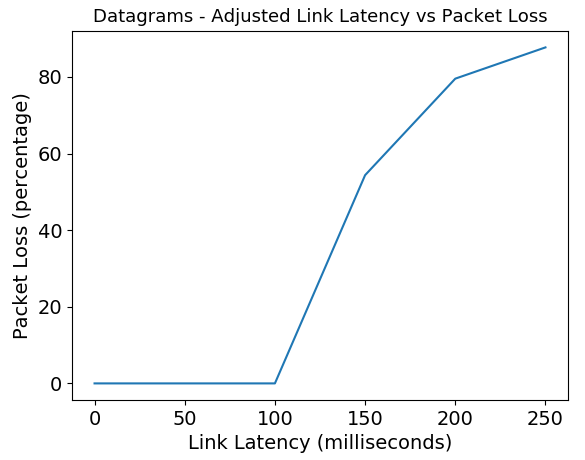
\includegraphics[width=0.475\linewidth]{images/latency/dg-lat-loss.png}
    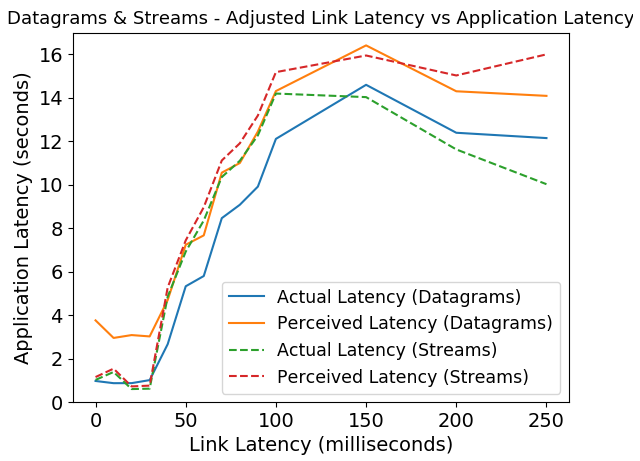
\includegraphics[width=0.515\linewidth]{images/latency/dg-streams-lat-lat.png}
    \caption{Left: Packet loss affected by link latency in our WebTransport Datagrams build. Right: Application latency affected by link latency in both WebTransport builds.}
    % use the notation fig:name to cross reference a figure
    \label{fig:dg-lat-loss-dg-streams-lat-lat} 
\end{figure}

WebRTC fared very well under high latency. As seen in Table \ref{tab:webrtc-lat}, there was no packet loss and there is no indication that decoding time was affected. Decoding time, once again, was very small. There was obviously a visible delay in the receiving video being displayed due to the link latency, but the image quality and smoothness were unaffected. A comparison of decoding time between all the builds can be seen in Figure \ref{fig:all-dec-lat}.

\begin{figure}[h]
    \centering
    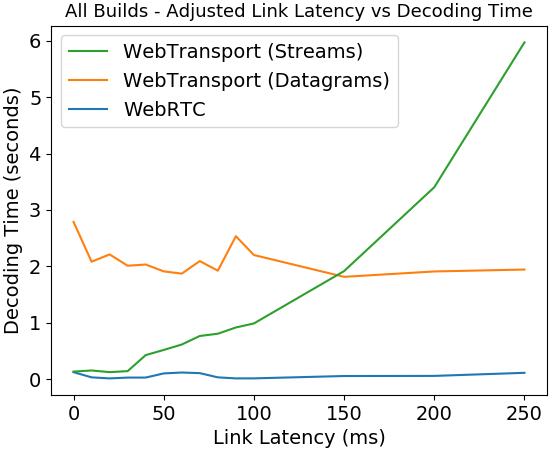
\includegraphics[width=0.6\linewidth]{images/latency/all-dec.png}
    \caption{All builds' decoding time against link latency mapped onto one graph.}
    % use the notation fig:name to cross reference a figure
    \label{fig:all-dec-lat} 
\end{figure}

Additionally, WebRTC does not suffer any packet loss even in high latency. However, the experiment failed after 500ms latency as the connection between the clients could no longer be established.

Overall, WebRTC greatly outperforms the WebTransport builds when adjusting latency. The Datagrams build is let down by its high decoding time and sensitivity to packet loss, and the Streams build suffers from comparatively high decoding times at high latencies. The WebRTC build maintains very low decoding time at all latencies and did not drop any packets during this experiment.
\hfill{} \\
\subsubsection{Experiment 3 - Adjusting Loss} 
\hfill{} \\
As seen in Table \ref{tab:wt-dg-loss}, our WebTransport Datagrams build results for this experiment were generally as expected. The build's packet loss percentage is usually approximately equal to the link loss multiplied by six - this is because we have six links in our network topology. This can be observed on the left of Figure \ref{fig:dg-loss-lat}. Because of this multiplication, experiments past 20\% link loss did not work as connection could not be established. 

% \begin{figure}[h]
%     \centering
%     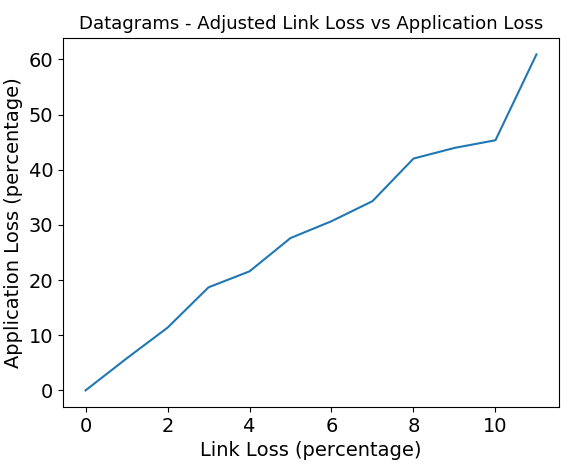
\includegraphics[width=0.6\linewidth]{images/loss/dg-loss-loss.png}
%     \caption{Adjusted link loss' effect on packet loss in our WebTransport Datagrams build.}
%     % use the notation fig:name to cross reference a figure
%     \label{fig:dg-loss-loss} 
% \end{figure}

As seen on the right in Figure \ref{fig:dg-loss-lat}, perceived latency is slightly lower than in our other experiments - this is because our packet handling mechanisms often discarded frames with heavy packet loss and rendered them as incomplete frames. Because of this, although the received video may have been relatively smooth, the image quality quickly became very poor. In general, the decoding time stays between approximately 2-3 seconds with some small outliers.

\begin{figure}[h]
    \centering
    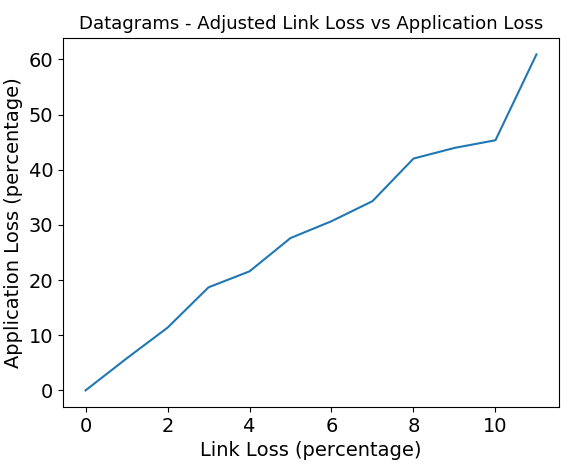
\includegraphics[width=0.49\linewidth]{images/loss/dg-loss-loss.png}
    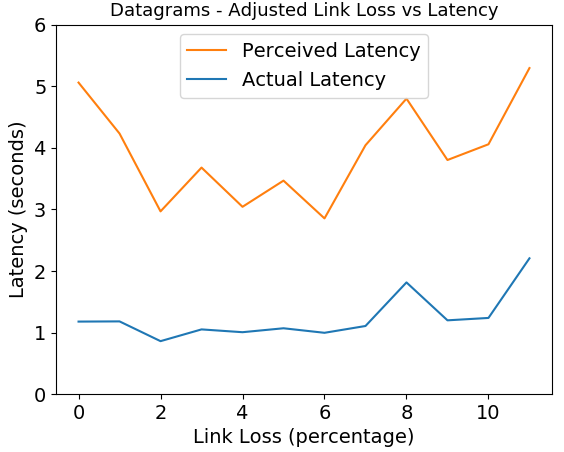
\includegraphics[width=0.49\linewidth]{images/loss/dg-loss-lat.png}
    \caption{Left: Adjusted link loss' effect on packet loss in our WebTransport Datagrams build. Right: Adjusted link loss' effect on latencies in our WebTransport Datagrams build.}
    % use the notation fig:name to cross reference a figure
    \label{fig:dg-loss-lat} 
\end{figure}

The results from the experiment on our Streams build can be seen in Table \ref{tab:wt-streams-loss}. As we can see, the experiments did not function past 12\% link loss rate here. This is surprising since streams are lossless, but it seems that the connection to the server timed out during connection establishment as packets were being retransmitted. Aside from this, results indicate that the Streams build functions adequately with high link loss rate. Decoding time does increase with loss rate - this is expected as the client must wait for packets to be retransmitted before completing a frame, and higher loss results in more retransmissions. Decoding time is relatively low, but still does rise alongside our link loss rate. This is once again because lost packets need to be retransmitted, thus stalling frame processing and increasing decoding time. However, as our links have very low latency, this does not have a significant effect on our decoding time as packets are quickly retransmitted. There is no solid discernible trend with our actual and perceived latencies - it does appear that with higher loss rates, we are more likely to see higher latencies, but there are too many outliers to state that there is a direct relationship between link loss rate, actual latency and perceived latency.

Our WebRTC build functioned well with high loss, as seen in Table \ref{tab:wrtc-loss}. Once again, these experiments were not able to progress past 20\% link loss rate as connection establishment failed. 
Surprisingly, the WebRTC build suffered no packet loss. This is because of WebRTC's forward error correction mechanisms. Indeed, more frames were dropped than usual in comparison to other WebRTC experiments, as they were likely "timed out" as packets were being retransmitted, but image quality and smoothness never appeared to decline or lag. Furthermore, decoding time once again stayed very consistent and appeared to be unaffected by link loss rate.

In the left of Figure \ref{fig:dg-nwq-loss}, we can see each build's decoding time mapped onto one graph.

% \begin{figure}[h]
%     \centering
%     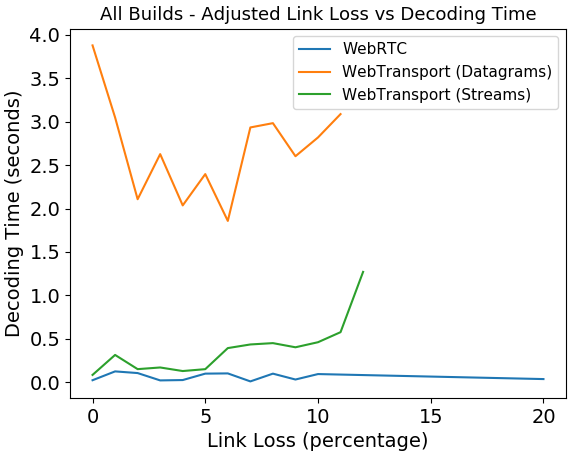
\includegraphics[width=0.6\linewidth]{images/loss/all-loss-decode.png}
%     \caption{All builds' decoding time against link loss rate mapped onto one graph.}
%     % use the notation fig:name to cross reference a figure
%     \label{fig:all-dec-loss} 
% \end{figure}

From this and our previous results, we can determine that our Datagrams build is by far the worst at dealing with loss. Our Streams build functions well at low loss rates but begins to suffer at higher loss rates, and WebRTC deals with loss extremely well.

\hfill{} \\
\subsubsection{Experiment 4 - Adjusting Network Quality (Bandwidth, Latency and Loss)} 
\hfill{} \\
In this experiment, all builds behave as expected. It should be noted that, as before, experiments only ran certain amounts of configuration numbers due to connection establishment issues: our Datagrams build ran 13, our Streams build ran 10 and our WebRTC build ran 20. The data for this experiment can be viewed in Table \ref{tab:wt-dg-nwq}. The most significant effects discovered in the previous experiments are exacerbated here by the other metrics in each configuration. For example, the Datagrams build's packet loss follows a similar pattern to the loss discovered in our Latency experiment (seen in the left of Figure \ref{fig:dg-lat-loss-dg-streams-lat-lat}), but it occurs at a far earlier latency. Instead of spiking at 150ms like before, the extreme packet loss occurs at a latency of 37.5ms (or independent variable Configuration 4); this is because of this configuration's corresponding link loss value of 1.5\% further worsening the existing packet loss. This effect can be seen in the right of Figure \ref{fig:dg-nwq-loss}.

\begin{figure}[h]
    \centering
    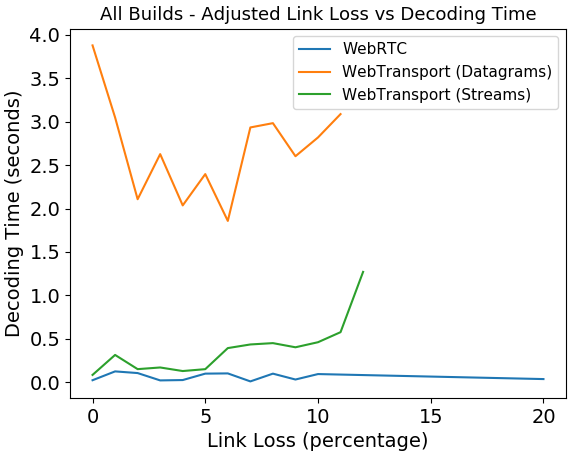
\includegraphics[width=0.49\linewidth]{images/loss/all-loss-decode.png}
    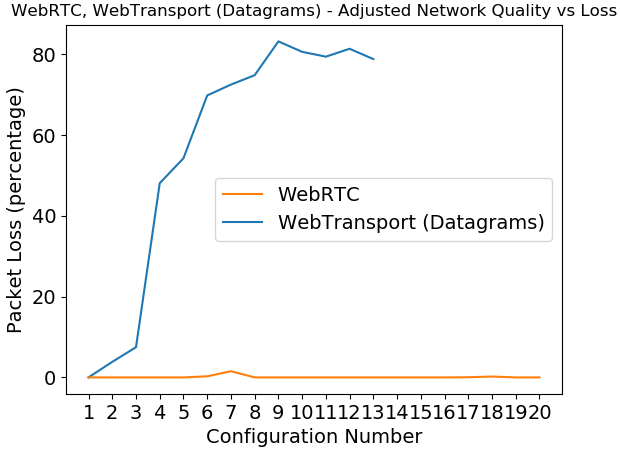
\includegraphics[width=0.49\linewidth]{images/combo/dg-nwq-loss.png}
    \caption{Left: All builds' decoding time against link loss rate mapped onto one graph. Right: The effect of our network quality configurations on WebTransport (Datagrams) and WebRTC builds' packet loss.}
    % use the notation fig:name to cross reference a figure
    \label{fig:dg-nwq-loss} 
\end{figure}

Another notable effect from previous experiments that is worsened here is latency's and loss' effects on our Streams build's decoding time. In our Latency experiment, the Streams build's decoding time became worse than our Datagrams build's at a link latency of 150ms - this can be seen in Figure \ref{fig:all-dec-lat}. In this experiment, this same thing occurs at a link latency of 62.5ms (or at Configuration 6). This can be observed on the left in Figure \ref{fig:all-nwq-dec}. This happens due to the effect link latency has on the WebTransport Streams build's decoding time being combined with the effect link loss rate has on it - more packets are lost and so total retransmission time increases, thus increasing decoding time.

\begin{figure}[h]
    \centering
    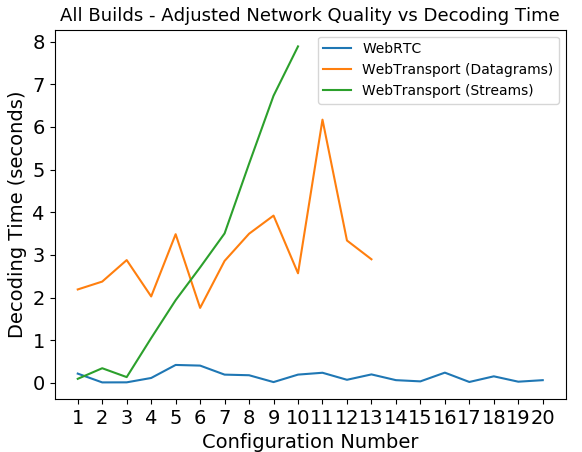
\includegraphics[width=0.49\linewidth]{images/combo/all-nwq-dec.png}
    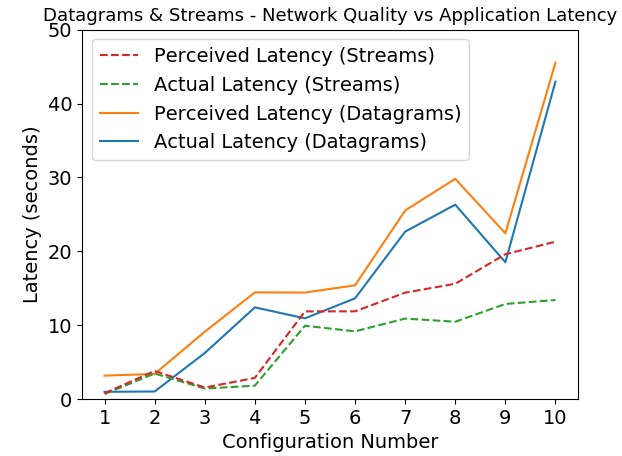
\includegraphics[width=0.49\linewidth]{images/combo/dg-streams-nwq-lat.png}
    \caption{Left: All builds’ decoding time against our adjusted network quality configurations mapped onto one graph. Right: Application latency affected by realistic network conditions in both WebTransport builds.}
    % use the notation fig:name to cross reference a figure
    \label{fig:all-nwq-dec} 
\end{figure}

Despite this poor decoding time, our Streams build still outperforms our Datagrams build due to the latter's previous issues with actual and perceived latencies reoccurring in this experiment. These two metrics are at the worst we have seen them by far, indicating that our Datagrams build does not perform well at all in realistic network conditions. This can be seen on the right in Figure \ref{fig:all-nwq-dec}.

% \begin{figure}[h]
%     \centering
%     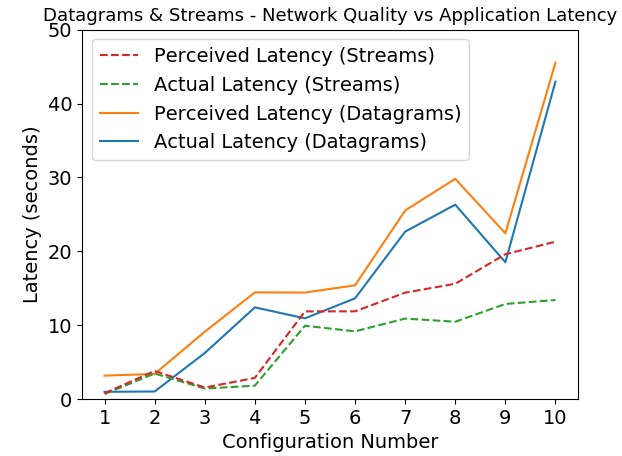
\includegraphics[width=0.6\linewidth]{images/combo/dg-streams-nwq-lat.png}
%     \caption{Application latency affected by realistic network conditions in both WebTransport builds.}
%     % use the notation fig:name to cross reference a figure
%     \label{fig:dg-streams-nwq-lat} 
% \end{figure}

Our WebRTC build performed well. As seen on the left in Figure \ref{fig:all-nwq-dec}, it once again maintained a very good decoding time throughout the experiment, resulting in high quality and smooth video playback. One interesting thing to note is that this experiment was the only one in which we noticed some packet loss (seen in the right of Figure \ref{fig:dg-nwq-loss}) - however, the amount of packets lost is relatively minuscule and there was no perceivable effect on image quality or smoothness. 

The main conclusion from this experiment is that all of the negative effects due to individual metrics observed in our previous experiments are exacerbated when combined into one simulated network. Our WebRTC build once again outperforms our WebTransport builds, and our Streams build generally outperforms its Datagrams counterpart. The Datagrams build suffers significantly in all configurations excluding the first one (where the network conditions are perfect), indicating that it does not perform well in realistic network conditions.

\hfill{} \\
\subsubsection{Experiment 5 - Adjusting CPU Usage} 
\hfill{} \\
Our WebTransport Datagrams build suffers a lot from varying CPU usage of the clients. Results for this can be seen in Table \ref{tab:wt-dg-cpu}. There are no apparent trends here, but it is evident to see that even dropping each client to using 90\% of available CPU resources causes our latencies and decoding time to increase significantly. Actual latency, perceived latency and our decoding times all vary significantly in seemingly random fashion. This indicates that our Datagrams build heavily relies on a powerful machine to render frames in a timely manner. Packet loss, however, does not appear to be significantly affected. Image quality and smoothness varies from good to unrecognisable. 

Our WebTransport Streams build handles varying CPU usage comparatively well. Results here can be seen in Table \ref{tab:wt-streams-cpu}. Similarly to previous experiments, actual and perceived latency increase as CPU usage gets to extremely low values, but not nearly to the same extent as our Datagrams build. We can see the latencies of our two WebTransport builds in Figure \ref{fig:dg-streams-cpu-lat}. Decoding time also increases slightly alongside the latencies, but is generally low enough to be adequate. In general, image quality and smoothness is good, but smoothness degrades with the extremely low CPU usage values.

\begin{figure}[h]
    \centering
    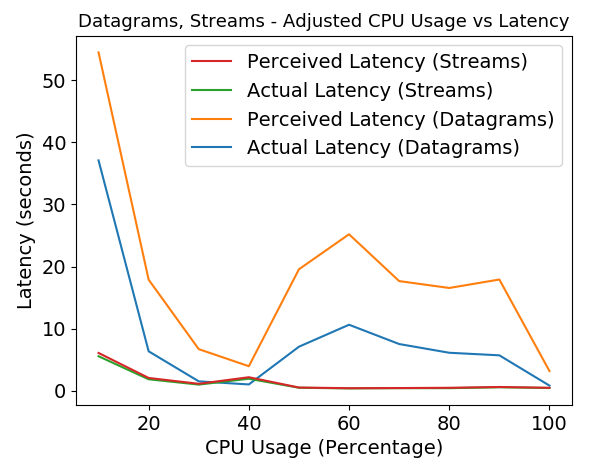
\includegraphics[width=0.6\linewidth]{images/cpu/dg-streams-cpu-lat.png}
    \caption{Application latencies affected by CPU usage in both WebTransport builds.}
    % use the notation fig:name to cross reference a figure
    \label{fig:dg-streams-cpu-lat} 
\end{figure}

The WebRTC build performed extremely well - CPU usage appears to have no effect on the build's performance in any regard. However, it should be noted that the WebRTC build failed to launch at 20\% and 10\% CPU usage, so we were unable to evaluate the metrics at these values. The results from this experiment can be seen in Table \ref{tab:wrtc-cpu}.

We can see the decoding time of all builds against CPU usage on the left in Figure \ref{fig:all-dec-cpu}, and just our Streams build against our WebRTC build on the right.

\begin{figure}[h]
    \centering
    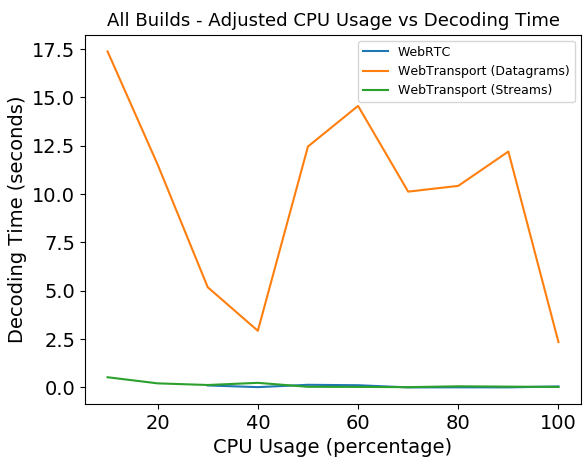
\includegraphics[width=0.49\linewidth]{images/cpu/all-cpu-decode.png}
    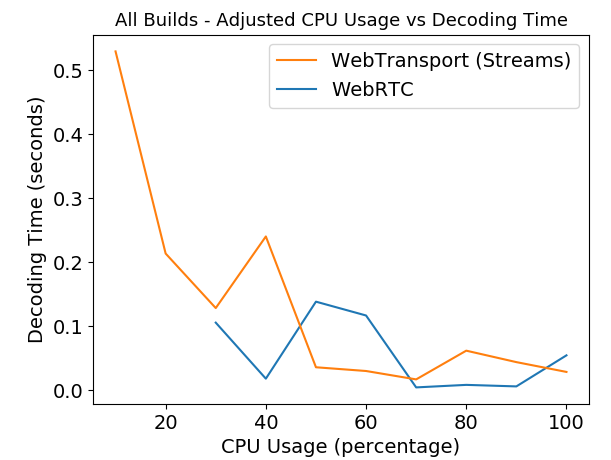
\includegraphics[width=0.49\linewidth]{images/cpu/wrtc-streams-cpu-decode.png}
    \caption{Left: builds' decoding time against CPU usage mapped onto one graph. Right: The WebTransport Streams and WebRTC builds' decoding time against CPU usage.}
    % use the notation fig:name to cross reference a figure
    \label{fig:all-dec-cpu} 
\end{figure}

As we can see on the left figure, our Datagrams build is clearly the worst-performing with regards to decoding time. On the right figure, we see that our Streams build and our WebRTC build perform similarly - any difference is negligible as the decoding time values are so small. Although WebRTC does appear to be slightly better, we cannot conclusively state this as we do not know what would have happened had the experiment run when CPU Usage was 10\% and 20\%.  

Overall, it is clear that our Datagrams build is heavily affected by varying CPU usage and would not perform well on less powerful devices; this is likely due to the inefficient algorithms that handle packet disorder and loss. Our Streams build is only slightly affected, and our WebRTC build does not appear to be affected at all (although this may not be the case in extremely low CPU usage percentages).

\hfill{} \\
\subsubsection{Overall Experiments Results} 
\hfill{} \\

Overall, it is clear that WebRTC outperforms both our WebTransport builds. Poor network quality barely affects it, and image quality and smoothness is almost always good. 

On the whole, our Streams build performs better than our Datagrams build. The Streams build does suffer in extremely poor network conditions, particularly when link latency and loss are high; such conditions result in long decoding times and video output that is not smooth. The build performs well in our good and average network conditions, but the image quality and smoothness is never as good as our WebRTC build simply because data transfer via streams is too slow.

Our Datagrams build has two main points of failure: the algorithms that handle packet loss and disorder, and the lack of mechanisms to negate packet loss in the first place. Evidence of the former is the results returned from our actual latencies, perceived latencies and decoding times. The reason that actual latency is high is that the client cannot start processing another frame until it has finished processing the current frame - when CPU usage or network conditions are poor, it takes far longer to process each frame and the perceived latency increases, consequently resulting in the perceived latency of the next frame to increase. The algorithms that handle packet disorder and loss are not robust at all and heavily rely on good network conditions and CPU usage. There are several ways that these algorithms could be improved; we would suggest utilising a more efficient data structure for the queues, dynamically varying the timeout for discarding frames and implementing some sort of multithreading functionality that continues to receive and process packets whilst our queue is being managed.
Evidence of poor loss management can be seen in the differences of packet loss statistics between our Datagrams and WebRTC builds. Despite both delivering packets in an unreliable fashion, WebRTC almost never loses packets, whereas our Datagrams build does so regularly. If we were to implement, for example, forward error correction mechanisms in our Datagrams build to the same standard as WebRTC's implementation, we may see heavily reduced packet loss which would in turn reduce the strain on our previously discussed packet handling algorithms.

Our Streams build performing better than its Datagrams counterpart was unexpected as datagrams' timely nature is theoretically better for video conferencing applications. However, the Streams build does not have much room for improvement - additional tweaks may slightly improve performance, but it is very unlikely that it is technically possible to be as good as WebRTC. However, as evidenced by these experiments, the Datagrams build does have a lot of room for improvement - we believe that it could theoretically outperform WebRTC due to WebTransport's support for developer freedom and utilisation of QUIC. If steps were taken to address the two main weaknesses outlined above, it would be interesting to reevaluate these builds and see if WebTransport could be used to its full potential.

These results prove that we have quantitatively evaluated the performance of several builds of a simple video conferencing application using different APIs (WebTransport and WebRTC) and data transfer methods, thus achieving the main goal of this project.
\hfill{} \\
\subsection{User Survey}
Our user survey generally backs up the findings from our experiments. For the survey, we gathered 25 anonymised participants from a range of ages and technical abilities.

In Table \ref{tab:likert-responses}, we can observe the average results of the responses to our Likert scale questions concerning the image quality, video smoothness and overall quality of each build. These Likert scale questions were from 1-5, with 1 being the lower end of the scale and 5 being the higher; we calculated the average result from each answer by totalling the responses (with a response of "4" for example being equal to 4 points) and dividing by 25 (the total number of participants). 

\begin{table}[H]
\centering
\resizebox{\textwidth}{!}{%
\begin{tabular}{lllll}
\hline
Build                                     & Avg. Quality & Avg. Smoothness & Avg. Overall &  \\ \hline
Alpha (WebTransport Datagrams)            & 2.52         & 1.12            & 1.76         &  \\
Beta (WebRTC)                             & 4.44         & 4.68            & 4.64         &  \\
Charlie (WebTransport Streams)            & 2.28         & 1.32            & 1.64         &  \\
Delta (WebTransport Datagrams  - Mininet) & 2            & 1.24            & 1.44         &  \\
Echo (WebRTC - Mininet)                   & 3.92         & 3.44            & 3.36         &  \\
Foxtrot (WebTransport Streams - Mininet)  & 2.44         & 1.56            & 1.84         &  \\ \hline
\end{tabular}%
}
\caption{Participant responses to our survey's Likert scale questions.}
\label{tab:likert-responses}
\end{table}

Before discussing these results, we shall display the outcome for our final question asking participants to rank each build. The following graph (Figure \ref{fig:ranks}) was generated by assigning points to each build depending on what ranks they were given by each participant - 1st place results in a build receiving 6 points, 2nd place results in a build receiving 5 points and so on. Every participant's ranking is taken into account, meaning that a build can have a potential total of 150 points (25 participants x 6 points if a build is given 1st place by each participant).  

\begin{figure}[h]
    \centering
    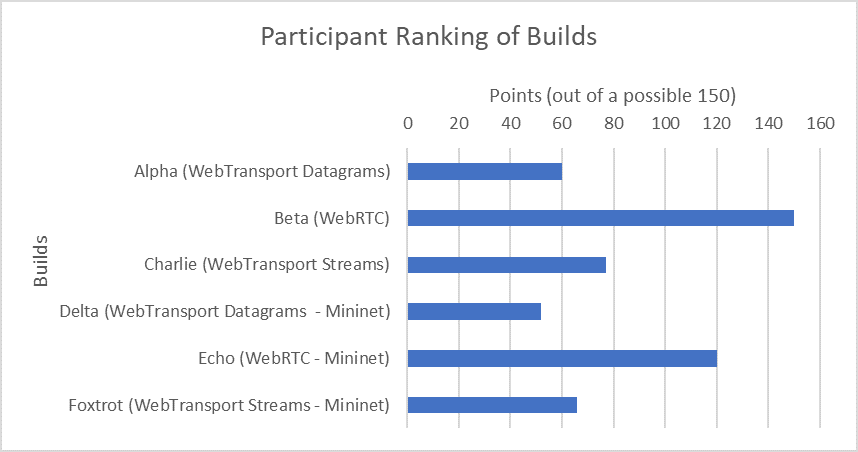
\includegraphics[width=0.73\linewidth]{images/user-survey-builds-rank.png}    

    \caption{Results calculated from participants' build rankings.}

    % use the notation fig:name to cross reference a figure
    \label{fig:ranks} 
\end{figure}

It is clear to see that our two WebRTC builds, Beta and Echo, proved to be the most well-received by our participants. In particular, participants unanimously responded that Beta was the highest-performing build across all metrics, with all participants ranking it as their highest build. Furthermore, Echo was second place in every question - this reflects our quantitative data that shows the WebRTC builds had generally better performance than the WebTransport ones.  

Our WebTransport builds had generally more mixed results, even when taking into account the "perfect" network conditions of Alpha and Charlie. Some of the results seem quite contradictory - for example, Foxtrot has a better average overall score than Charlie, but places worse in the final rankings. Additionally, Alpha has a better average overall score than Charlie, but once again places worse in the final rankings. This indicates that, in comparison to how the WebRTC builds scored and placed, there is less certainty about how the WebTransport builds perform with respect to each other. This is corroborated by feedback from four participants that stated it was difficult to tell the difference between the poorly-performing builds, as according to one participant, they were "just as bad as each other". Additionally, some participants stated that they were more certain of their answers when ranking the builds rather than when responding to the Likert scales - because of this, we have decided to assume that the final rankings are more indicative of apparent performance than the results from the Likert scale questions.

An important result to note is that participants were able to tell when network conditions affected quality - the three Mininet builds were each placed lower in the final rankings than their perfect network counterparts.

Finally, we can determine that, according to user observation, Streams builds perform better than Datagrams builds in both perfect network conditions and more realistic network conditions. This corroborates the data from our experiments.

From these results, we can clearly see that using different technologies and data transfer methods have a significant effect on the user experience. If we go by the final rankings, participants were successfully able to assess the quality of each build - this is evidenced by our experiment results (WebRTC being better than WebTransport, our Streams build being better than our Datagrams build) and by the fact that each Mininet build is ranked lower than their corresponding perfect network builds. A key question asked by this project was whether the extra development overhead of using WebTransport makes a difference to the user or not - it clearly does, although obviously not in the way we wanted as it has a negative effect. Had our WebTransport builds been of a closer quality to (or better than) our WebRTC builds, it would have been interesting to see if this distinction between the builds using the two APIs could still be made by end users, as this would perhaps indicate to us whether advocating for the continued development of WebTransport would even be worth it. However, as our WebTransport builds fall short in terms of performance, we feel that this particular question has not been answered by this project. We can, however, say that the extra development overhead was not worth it in this instance from a purely results-oriented standpoint, and the user responses in this survey confirmed that. Despite not answering the question presented in our secondary project aim, the user survey was still useful as it serves as further evidence of our experiment results. 


% \section{Guidance}
% \begin{itemize}
%     \item
%         Ask specific questions that address the general problem.
%     \item
%         Answer them with precise evidence (graphs, numbers, statistical
%         analysis, qualitative analysis).
%     \item
%         Be fair and be scientific.
%     \item
%         The key thing is to show that you know how to evaluate your work, not
%         that your work is the most amazing product ever.
% \end{itemize}

% \section{Evidence}
% Make sure you present your evidence well. Use appropriate visualisations, 
% reporting techniques and statistical analysis, as appropriate. The point is not
% to dump all the data you have but to present an argument well supported by evidence gathered.

% If you use numerical evidence, specify reasonable numbers of significant digits; don't state ``18.41141\% of users were successful'' if you only had 20 users. If you average \textit{anything}, present both a measure of central tendency (e.g. mean, median) \textit{and} a measure of spread (e.g. standard deviation, min/max, interquartile range).

% You can use \texttt{siunitx} to define units, space numbers neatly, and set the precision for the whole LaTeX document. 

% % setup siunitx to have two decimal places
% \sisetup{
% 	round-mode = places,
% 	round-precision = 2
% }

% For example, these numbers will appear with two decimal places: \num{3.141592}, \num{2.71828}, and this one will appear with reasonable spacing \num{1000000}.



% If you use statistical procedures, make sure you understand the process you are using,
% and that you check the required assumptions hold in your case. 

% If you visualise, follow the basic rules, as illustrated in Figure \ref{fig:boxplot}:
% \begin{itemize}
% \item Label everything correctly (axis, title, units).
% \item Caption thoroughly.
% \item Reference in text.
% \item \textbf{Include appropriate display of uncertainty (e.g. error bars, Box plot)}
% \item Minimize clutter.
% \end{itemize}

% See the file \texttt{guide\_to\_visualising.pdf} for further information and guidance.

% \begin{figure}[h]
%     \centering
%     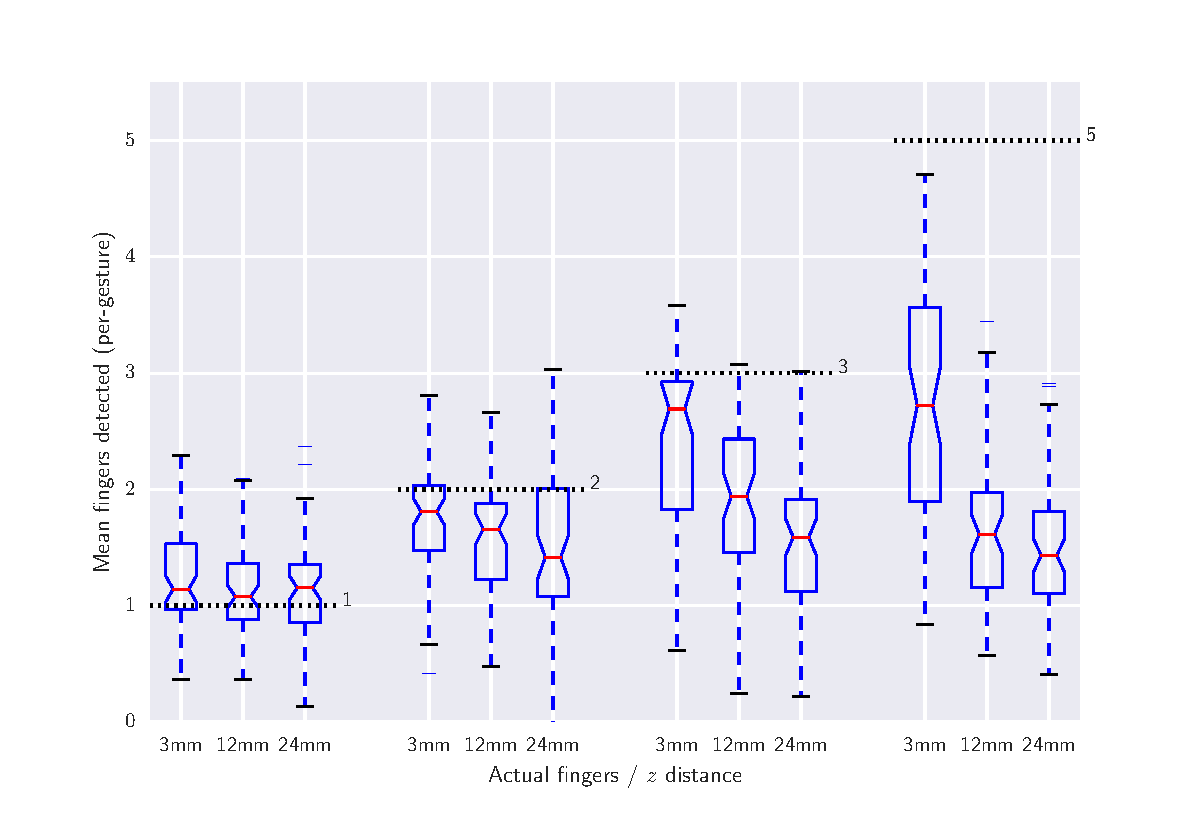
\includegraphics[width=1.0\linewidth]{images/boxplot_finger_distance.pdf}    

%     \caption{Average number of fingers detected by the touch sensor at different heights above the surface, averaged over all gestures. Dashed lines indicate
%     the true number of fingers present. The Box plots include bootstrapped uncertainty notches for the median. It is clear that the device is biased toward 
%     undercounting fingers, particularly at higher $z$ distances.
%     }

%     % use the notation fig:name to cross reference a figure
%     \label{fig:boxplot} 
% \end{figure}


% %==================================================================================================================================